\chapter{Introduction}
\label{chap:introduction}
Nowadays, \gls{lidar} sensors are widely used in various applications, including autonomous vehicles, robotics, and environmental mapping \cites[]{doubrava_LIDARSenzorJeho_2021}[Ch.~4-6]{dong_LiDARRemoteSensing_2017}.
While the former two applications often require high-end and expensive \gls{lidar} systems, environmental mapping can be effectively performed using more affordable sensors.
However, even the cheapest commercial 3D \gls{lidar} sensor, which was found during the research for this miniproject, costs 249~\euro \cite{_4DLidarL1_}.

This bachelor's thesis addresses two main objectives. The first objective is the development of a cost-effective platform for a $360\,\degree$ STL-19P \gls{lidar} sensor that enables 3D spatial scanning using a 2D \gls{lidar} sensor.
\begin{figure}[h]
    \centering
    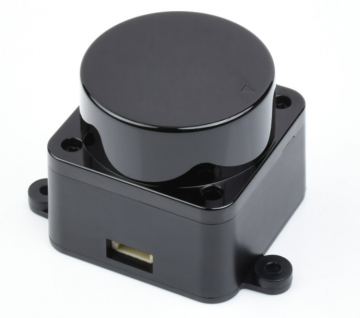
\includegraphics[width=0.5\textwidth]{introduction/lidar_photo.png}
    \caption{Photo of STL-19P \gls{lidar} \protect\footnotemark}
    \label{ph:lidar_photo}
\end{figure}
\begin{table}[h]
    \centering
    \caption{Main parameters of STL-19P \gls{lidar}\protect\footnotemark[1]}
    \rowcolors{0}{ctubluebg!65}{ctubluebg!20}
    \begin{tabular}{|c|c|}
        \toprule
        Typical measuring range [$\si{m}$] & 0,03--12 \\
        Angular resolution [$\degree$] & 0,72\\
        Dimensions (W x L x H) [$\si{mm,mm,mm}$] & $38,59 \times 38,59 \times 33,50$\\
        Communication interface & UART @ 230400 bps \\
        \bottomrule
    \end{tabular}
    \label{tab:lidar_params}
\end{table}
\footnotetext[1]{Photo and parameters were taken from \url{https://www.waveshare.com/wiki/D500_LiDAR_Kit}}

The second objective is the utilisation of hardware tools, such as the Raspberry Pi Pico 2 W microcontroller\footnote{\url{https://www.raspberrypi.com/products/raspberry-pi-pico-2/}} for data acquisition, and software tools, such as the Python library Open3D \cite{zhou_Open3DModernLibrary_2018} for the 3D scene reconstruction.